\documentclass{article}

\usepackage[utf8]{inputenc}
\usepackage[brazilian]{babel}
\usepackage{graphicx}
\usepackage{float}
\usepackage[pdftex]{hyperref}
\usepackage{epstopdf}
\usepackage{etoolbox}
\usepackage{amsmath}
\usepackage{amsfonts}
\usepackage{amssymb}
\usepackage{caption}
\usepackage{subcaption}
\usepackage{setspace}
\usepackage{tikz}

\patchcmd{\thebibliography}{\section*}{\section}{}{}
\newcommand{\R}{\ensuremath{\mathbb{R}}}
\newcommand{\Prob}{\ensuremath{\mathbb{P}}}
\newcommand{\K}{\ensuremath{\mathbb{K}}}
\newcommand{\U}{\ensuremath{\mathbb{U}}}
\newcommand{\N}{\ensuremath{\mathbb{N}}}
\newcommand{\Lg}{\ensuremath{\mathbb{L}}}
\newcommand{\T}{\ensuremath{\rm Tr}}
\newcommand{\sg}{{\sigma(x_k)}}

\newcommand{\G}{\ensuremath{\mathcal{G}}}
\newcommand{\F}{\ensuremath{\mathcal{F}}}
\newcommand{\C}{\ensuremath{\mathcal{C}}}
\newcommand{\E}{\ensuremath{\mathcal{E}}}
\newcommand{\Hn}{\ensuremath{\mathcal{H}}}
%\newcommand{\Hoo}{\ensuremath{\mathcal{H}_\infty}}
\newcommand{\Hop}{\ensuremath{\mathcal{H}_{op}}}
% --------------------------------------------------
\newtheorem{theo}{Teorema}
\newtheorem{exa}{Exemplo}
\newtheorem{lemm}{Lema}
\newtheorem{coro}{Corolário}
\newtheorem{defn}{Definição}[section]

%opening


\begin{document}

\begin{titlepage}
\begin{center}

\newcommand{\HRule}{\rule{\linewidth}{0.5mm}}
% Upper part of the page. The '~' is needed because \\
% only works if a paragraph has started.

\includegraphics[width=0.15\textwidth]{logounicamp.pdf}~\\[1cm]

\textsc{\LARGE Universidade Estadual de Campinas}\\[1.5cm]

\textsc{\Large Faculdade de Engenharia Mecânica}\\[0.5cm]

% Title
\HRule \\[0.4cm]
{ \huge \bfseries ES828 - Laboratório de Controle de Sistemas\\ \vspace{1cm} Relatório - Experimento 2 \\
\Large{Método de identificação de plantas eletrônicas} \\[0.4cm] }

\HRule \\[1.5cm]

% Author and supervisor
\begin{minipage}{0.6\textwidth}
\begin{flushleft} \large
\emph{Nome:}\\
Daniel Dello Russo Oliveira\\ Marcelli Tiemi Kian
\end{flushleft}
\end{minipage}
\begin{minipage}{0.2\textwidth}
\begin{flushright} \large
\emph{RA}\\ 101918\\
117892
\end{flushright}
\end{minipage}

\vfill

% Bottom of the page
{\large \today}

\end{center}
\end{titlepage}


\onehalfspacing
\section{Objetivos} 
O objetivo desse experimento é realizar a identificação de parâmetros de um sistema torcional composto por dois discos interligados por uma haste flexível acionados por um motor de corrente contínua,conforme modelo proposto no roteiro\cite{bb:roteiro}. As posições angulares dos discos são medidas por dois encoders, e o motor é acionado pelo modulador de largura de pulso (PWM).
	
\section{Modelo matemático}
O modelo problema é mostrado no esquema da figura \ref{fig:esqmotor} e está descrito pelas equações \ref{eq:eletrica}, \ref{eq:disco1} e \ref{eq:disco2}. Para este experimento, iremos considerar que o indutor é carregado instantaneamente, ou seja, que $L=0$. Também adotaremos as variáveis de estado do sistema como $x_1=\theta_1-\theta_2$, $x_2=\dot{\theta_1}$ e $x_3=\dot{\theta_2}$.

\begin{figure}[H]
	\centering
	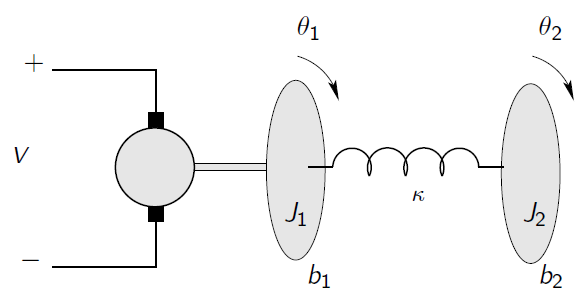
\includegraphics[width=0.8\linewidth]{esqmotor}
	\caption{Esquema do motor (elétrica e mecânica)}
	\label{fig:esqmotor}
\end{figure}

\begin{equation}
\label{eq:eletrica}
L\dot{i}+Ri+K\dot{\theta_1}=V
\end{equation}
\begin{equation}
\label{eq:disco1}
(J_1)\ddot{\theta_1}+b_1\dot{\theta_1}+\kappa(\theta_1-\theta_2)=Ki
\end{equation}
\begin{equation}
\label{eq:disco2}
(J_2)\ddot{\theta_2}+b_2\dot{\theta_2}+\kappa(\theta_2-\theta_1)=0
\end{equation}

\begin{equation}
\label{eq:ss}
\left[ \begin{array}{c}
\dot{x_1} \\
\dot{x_2} \\
\dot{x_3} \end{array} \right]
=
\left[ \begin{array}{ccc}
0 & 1 & -1 \\
-\frac{\kappa}{J_1} & -\frac{(b_1+K^2/R)}{J_1} & 0 \\
\frac{\kappa}{J_2} & 0 & -\frac{b_2}{J_2} \end{array} \right]
\left[ \begin{array}{c}
x_1 \\
x_2 \\
x_3  \end{array} \right]
+
\left[ \begin{array}{c}
0 				\\
\frac{K}{RJ_1} 	\\
0				\end{array} \right]
V

\end{equation}

\section{Ensaio com motor parado}
Conforme o roteiro\cite{bb:roteiro}, ao ligar o motor com o disco ligado a ele travado não geramos força contra-eletromotriz, e com isso conseguimos medir a corrente de armadura $i$ com a adição de um resistor $R_s$. Adotaremos a indutância $L=0$. Isso nos possibilita o cálculo do parâmetro $R [\Omega]$ (soma da resistência do motor e $R_s$) pela equação \ref{eq:rotparado}.

\begin{equation}
\label{eq:rotparado}
i(t) = \frac{V}{R}
\end{equation}

Travando o disco para impossibilitar o motor de girar seu rotor, fizemos o acionamento do módulo de potência, aguardamos a estabilização do sinal de corrente, e desligamento do sistema, obtendo a curva de corrente mostrada na figura \ref{fig:ensaiop}.

\begin{figure}[H]
	\centering
	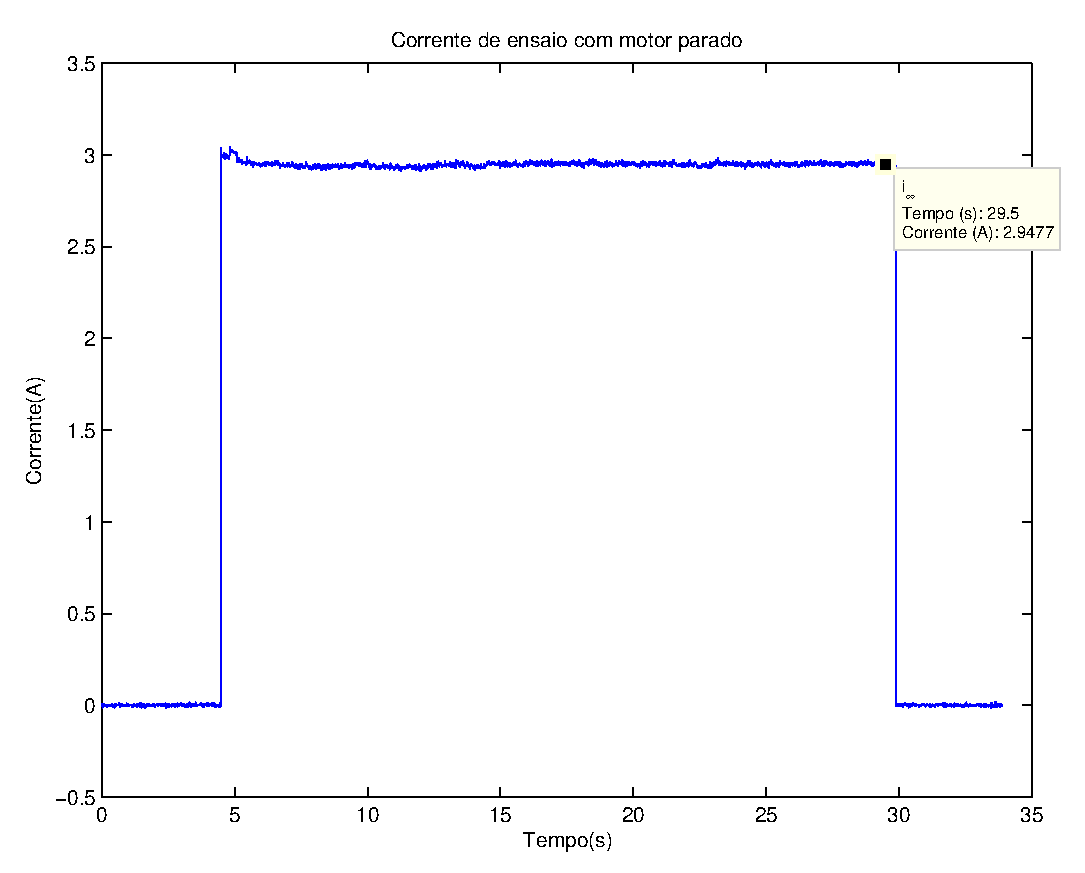
\includegraphics[width=0.8\linewidth]{../ensaiop}
	\caption{Corrente de ensaio com motor parado}
	\label{fig:ensaiop}
\end{figure}

Filtramos o sinal e destacamos alguns pontos mais relevantes para facilitar a análise, como pode ser visto na figura \ref{fig:riseI}.
\begin{figure}[H]
	\centering
	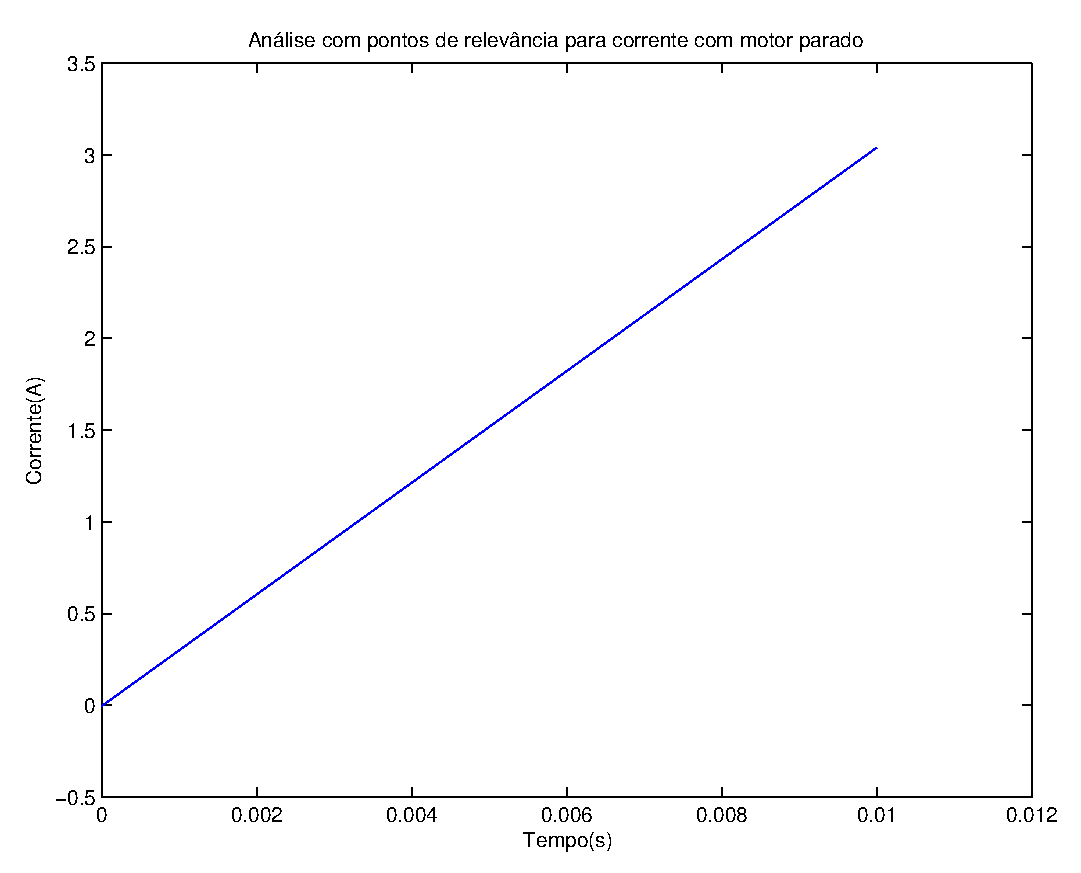
\includegraphics[width=0.8\linewidth]{../riseI}
	\caption{Pontos de relevância para corrente filtrada com motor parado}
	\label{fig:riseI}
\end{figure}

Para o cálculo do parâmetro $R$, utilizamos a tensão da fonte $V=12 V$ e a partir do momento em que a corrente se estabiliza em $i_\infty=%TODO: colocar a corrente de armadura
A$, calculamos seu valor conforme \ref{eq:r}.

\begin{equation}
\label{eq:r}
R = \frac{V}{i_\infty}=%TODO 11.2578\Omega
\end{equation}

\section{Ensaio com motor em movimento}
Agora sem travar o disco, acionamos o módulo de potência e aguardamos a estabilização do sinal de corrente e velocidade, e desligamos o sistema, obtendo a curva de corrente mostrada na figura \ref{fig:ensaiori} e a curva de velocidade angular mostrada na figura \ref{fig:ensaiorv}.

\begin{figure}[H]
	\centering
	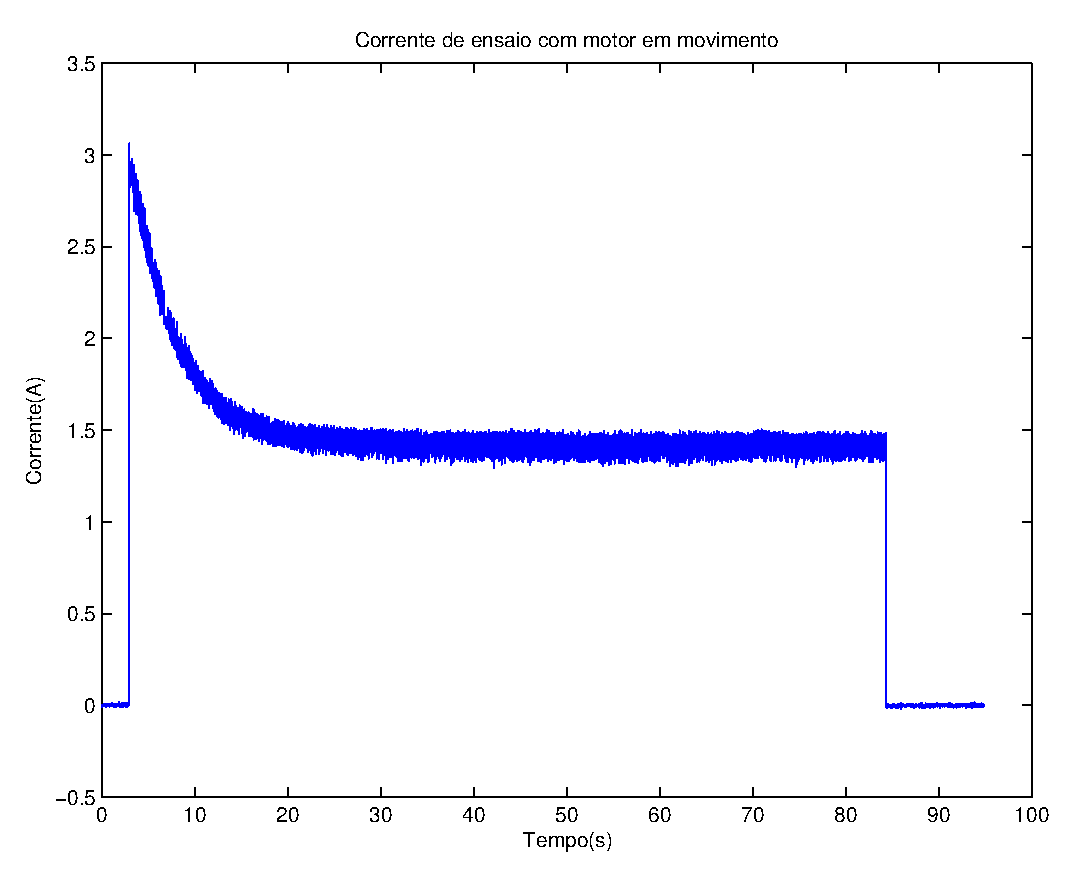
\includegraphics[width=0.8\linewidth]{../ensaiori}
	\caption{Corrente durante ensaio com motor em movimento}
	\label{fig:ensaiori}
\end{figure}

\begin{figure}[H]
	\centering
	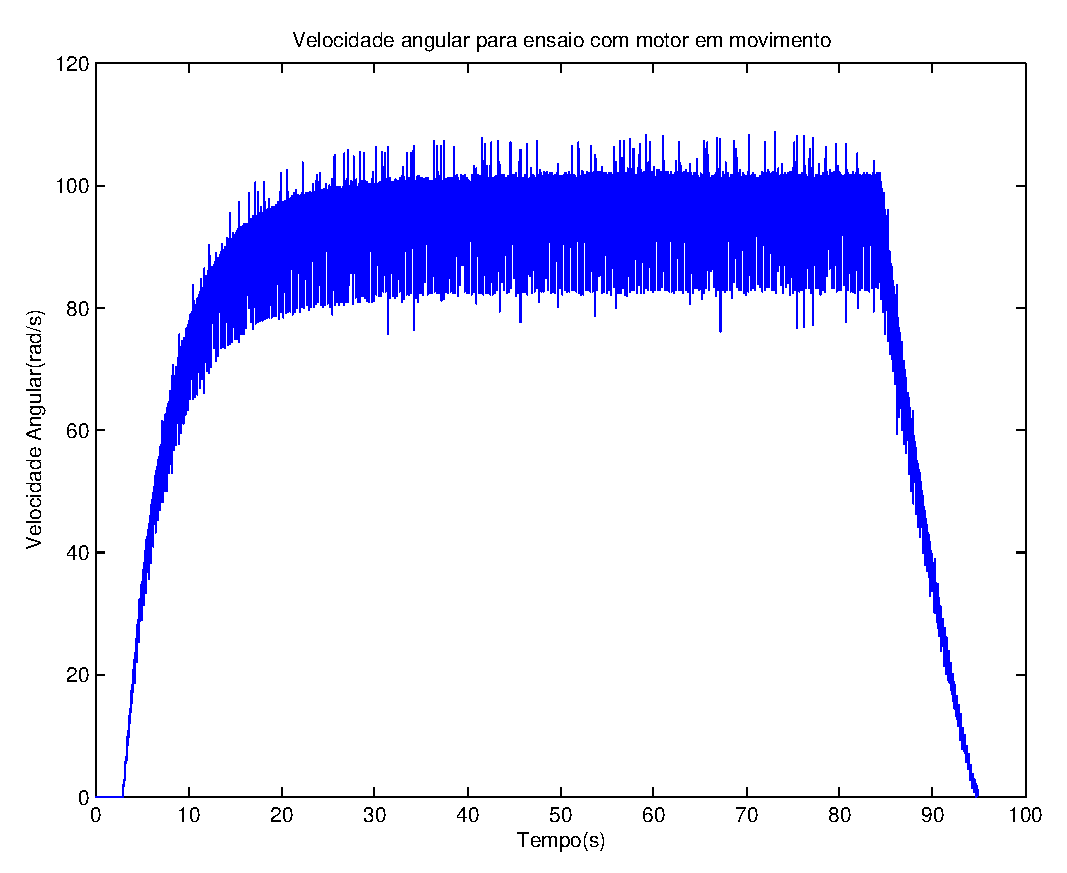
\includegraphics[width=0.8\linewidth]{../ensaiorv}
	\caption{Velocidade angular durante ensaio com motor em movimento}
	\label{fig:ensaiorv}
\end{figure}

Filtramos o sinal e destacamos alguns pontos mais relevantes para facilitar a análise, como pode ser visto nas figuras \ref{fig:ensaioriF} e \ref{fig:ensaiorvF}.
\begin{figure}[H]
	\centering
	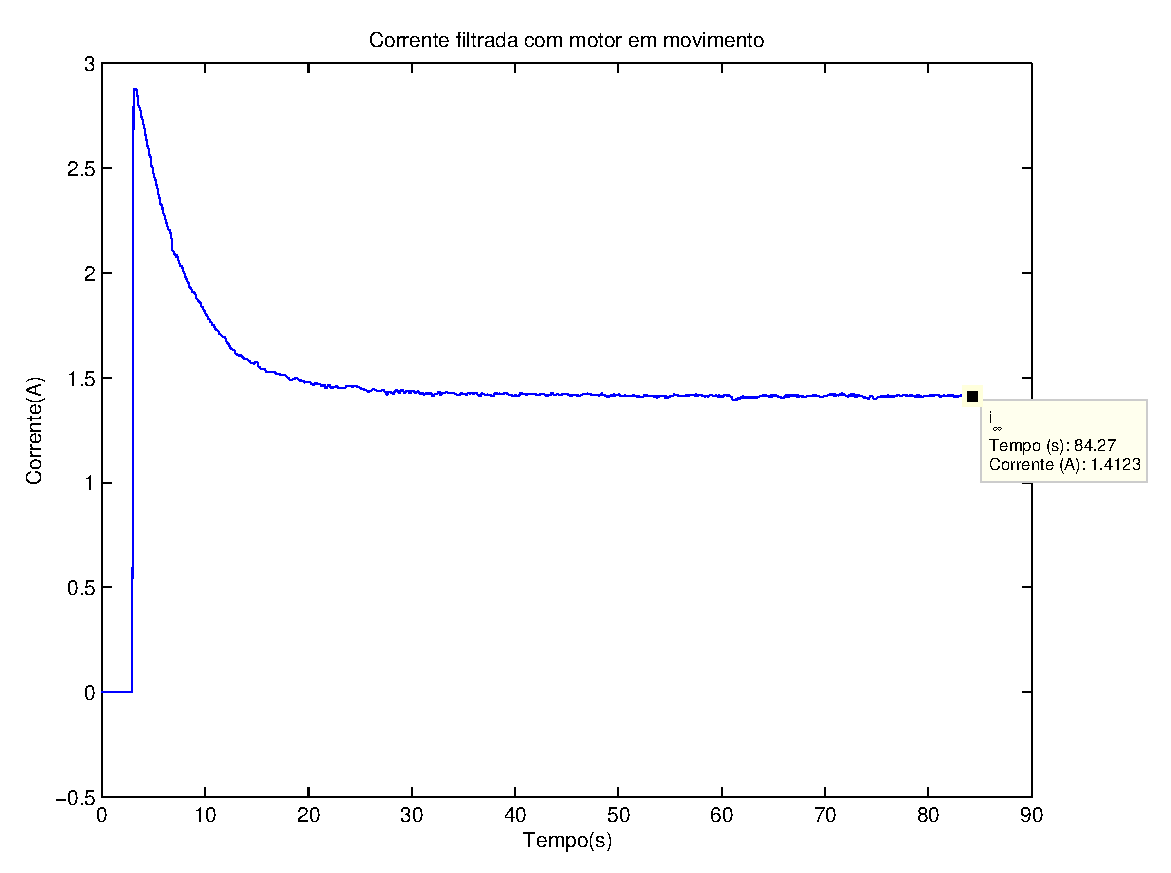
\includegraphics[width=0.8\linewidth]{../ensaioriF}
	\caption{Pontos de relevância para corrente filtrada com motor em movimento}
	\label{fig:ensaioriF}
\end{figure}

\begin{figure}[H]
	\centering
	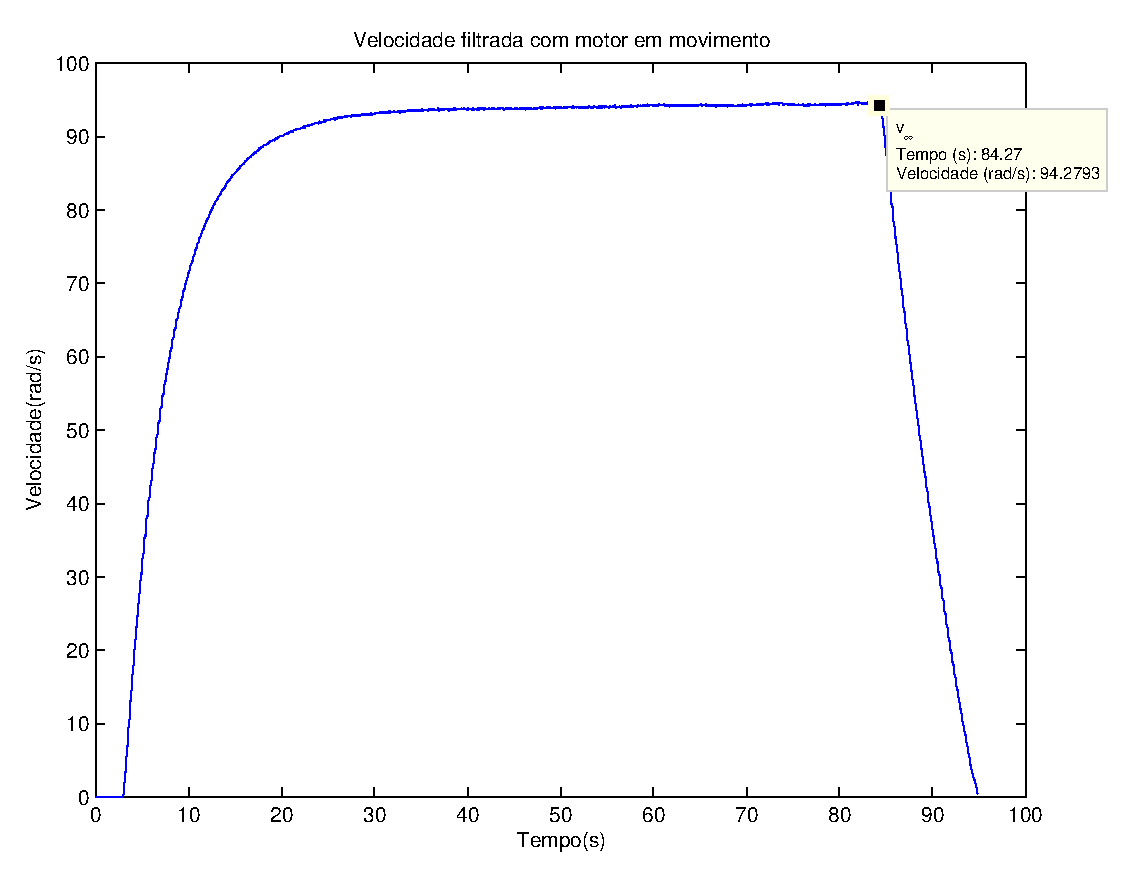
\includegraphics[width=0.8\linewidth]{../ensaiorvF}
	\caption{Pontos de relevância para velocidade angular filtrada com motor em movimento}
	\label{fig:ensaiorvF}
\end{figure}

Esperando a velocidade do motor se estabilizar, chegamos em $\nu_{\infty}=%TODO: Velocidade angular RP 155.3764rad/s
$. Considerando que a esse ponto o indutor se comporte como curto circuito, encontramos a constante de torque do motor conforme a equação \ref{eq:k}

\begin{equation}
\label{eq:k}
K=\frac{V-Ri_{\infty}}{\nu_{\infty}}=%TODO 0.0499 V.s
\end{equation}







Para encontrar o coeficiente de atrito viscoso $b$, utilizamos a equação \ref{eq:mecanica} aplicando a transformada de Laplace e utilizando o teorema do valor final, chegando à equação \ref{eq:b} para o cálculo.

\begin{equation}
\label{eq:b}
b=\frac{Ki_{\infty}}{\nu_{\infty}}=0.00011117 N.m.s
\end{equation}

Com a velocidade estabilizada, desligando a alimentação do motor, conseguimos calcular a constante de tempo $\tau_m=29.6943s$ em que $\nu(\tau_m)=0.3679\nu_{\infty}$. Depois, encontramos $J$ de acordo com a equação \ref{eq:j}.

\begin{equation}
\label{eq:j}
J=\tau_mb=0.0033 kg.m^2
\end{equation}

\section{Resultados finais}
Com todos os parâmetros necessários calculados, substituindo os valores em \ref{eq:gss}, obtemos a planta dada pela equação \ref{eq:gs}.

\begin{equation}
\label{eq:gs}
G(s)=\frac{10.42}{s^2 + 8.478s + 0.805}
\end{equation}

Essa planta pode ser representada na forma de estados pela equação \ref{eq:states}, substituindo os parâmetros pelos valores calculados temos a equação \ref{eq:statesval}:
\begin{equation}
\label{eq:states}
\begin{Bmatrix}
\dot{i}\\ \dot{\nu} \\ \dot{\Theta} 
\end{Bmatrix} =
\begin{bmatrix}
-\frac{R+R_s}{L} & -\frac{K}{L} & 0\\
\frac{K}{b} & -\frac{b}{J} & 0\\
0 & 1 & 0
\end{bmatrix}
\begin{Bmatrix}
i\\ \nu \\ \Theta 
\end{Bmatrix} + 
\begin{bmatrix}
\frac{1}{L} & 0 & 0\\
\end{bmatrix}
\begin{Bmatrix}
V 
\end{Bmatrix}
\end{equation}

\begin{equation}
\label{eq:statesval}
\begin{Bmatrix}
\dot{i}\\ \dot{\nu} \\ \dot{\Theta} 
\end{Bmatrix} =
\begin{bmatrix}
-8.4441 & -0.0344 & 0\\
15.1303 & -0.0337 & 0\\
0 & 1 & 0
\end{bmatrix}
\begin{Bmatrix}
i\\ \nu \\ \Theta 
\end{Bmatrix} + 
\begin{bmatrix}
0.6889 & 0 & 0\\
\end{bmatrix}
\begin{Bmatrix}
V 
\end{Bmatrix}
\end{equation}

Com o auxílio do matlab, simulamos esse sistema a comparamos os resultados dessa simulação com os dados adquiridos durante o ensaio com o motor em movimento. Essa comparação pode ser vista nas figuras \ref{fig:simi} e \ref{fig:simv}.
\begin{figure}[H]
	\centering
	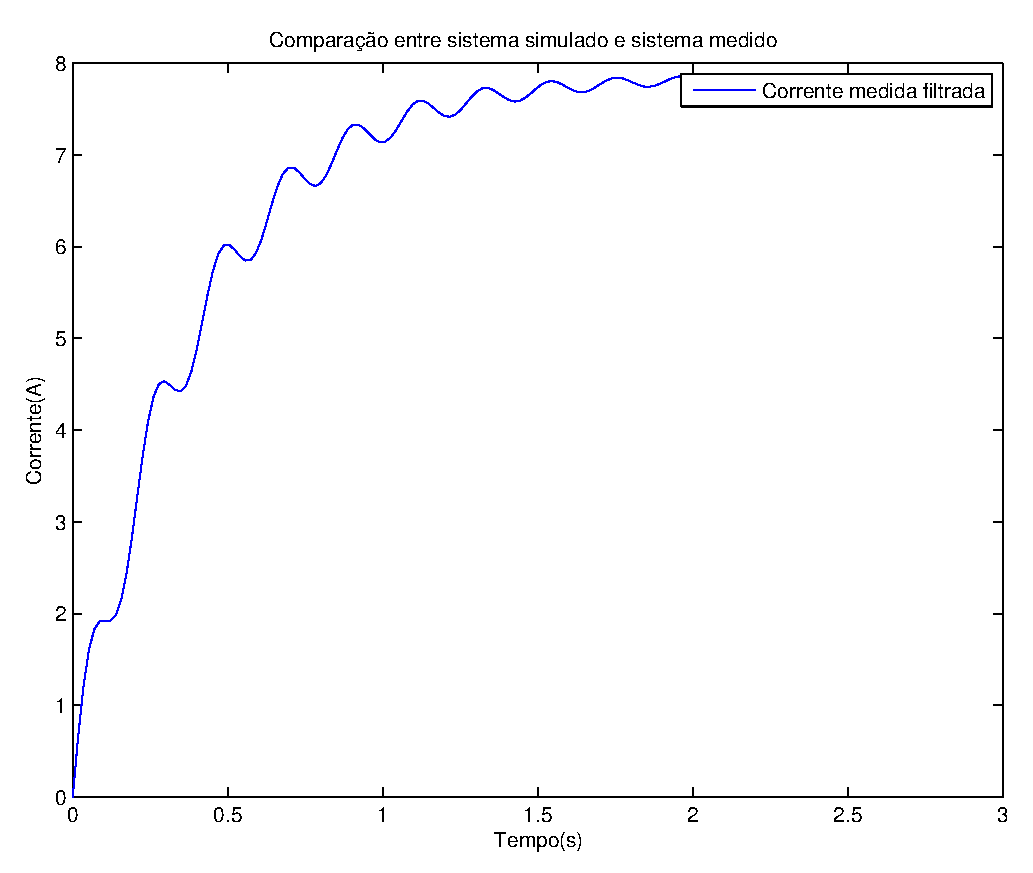
\includegraphics[width=0.8\linewidth]{../simi}
	\caption{Comparação entre corrente medida e simulada}
	\label{fig:simi}
\end{figure}
\begin{figure}[H]
	\centering
	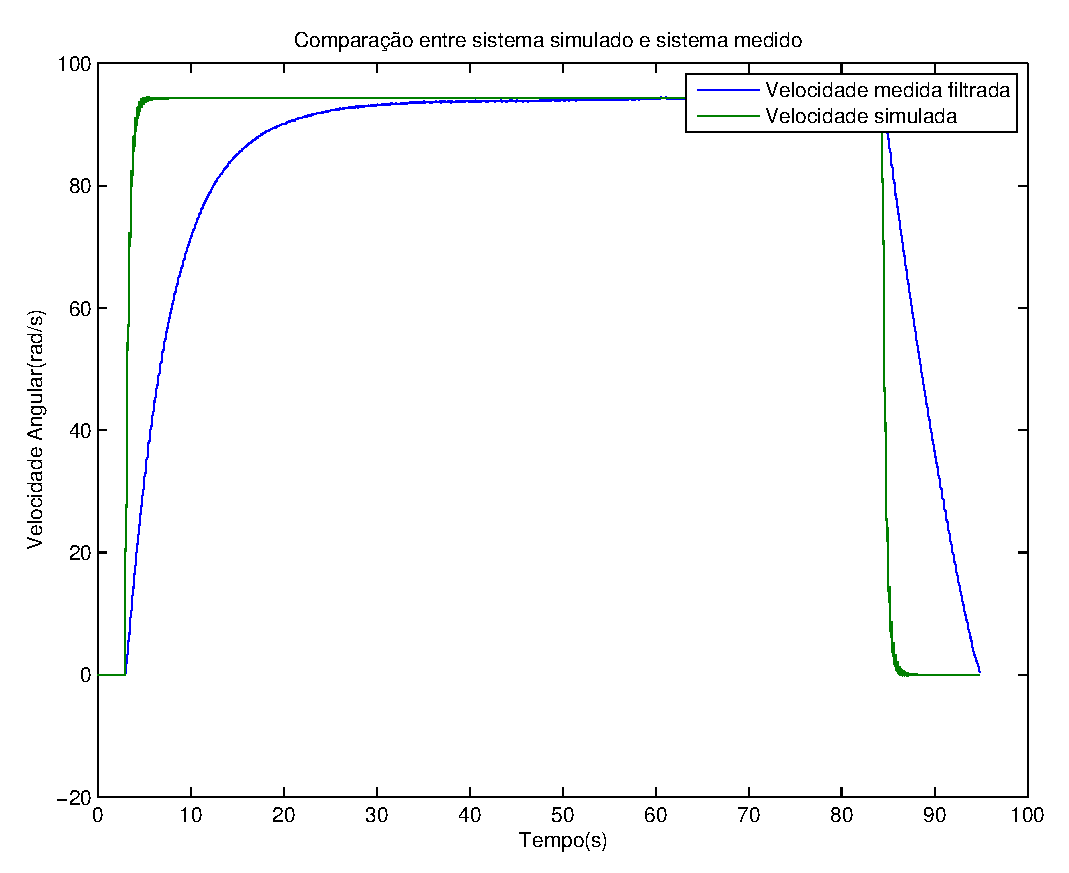
\includegraphics[width=0.8\linewidth]{../simv}
	\caption{Comparação entre velocidade angular medida e simulada}
	\label{fig:simv}
\end{figure}

A primeira coisa que notamos é que a corrente simulada apresenta um comportamento bastante diferente na queda, assumindo valores negativos. Acreditamos que o motivo dessa diferença seja a ponte H ligada no sistema, que deve se utilizar de diodos para proteger suas chaves de correntes e tensões reversas geradas pelo motor. Isso afeta significativamente a curva de decida da velocidade, tornando questionável a precisão do resultado obtido para $\tau_m$ e consequentemente do momento de inércia $J$.

Utilizamos então o Simulink para verificar o efeito dessa limitação de corrente no sistema. Para isso, impomos a mesma limitação no sistema simulado e obtivemos as curvas mostradas nas figuras \ref{fig:simisat} e \ref{fig:simvsat}.

\begin{figure}[H]
	\centering
	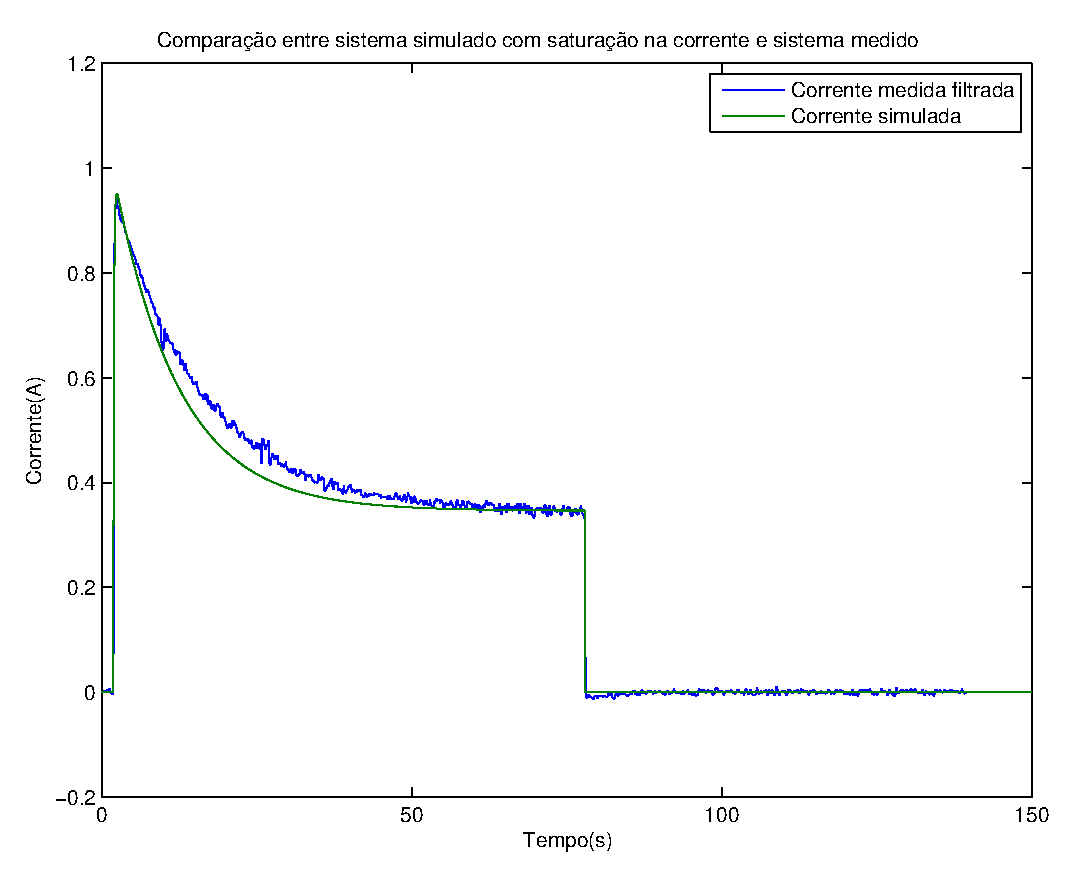
\includegraphics[width=0.8\linewidth]{../simisat}
	\caption{Comparação entre corrente medida e simulada}
	\label{fig:simisat}
\end{figure}
\begin{figure}[H]
	\centering
	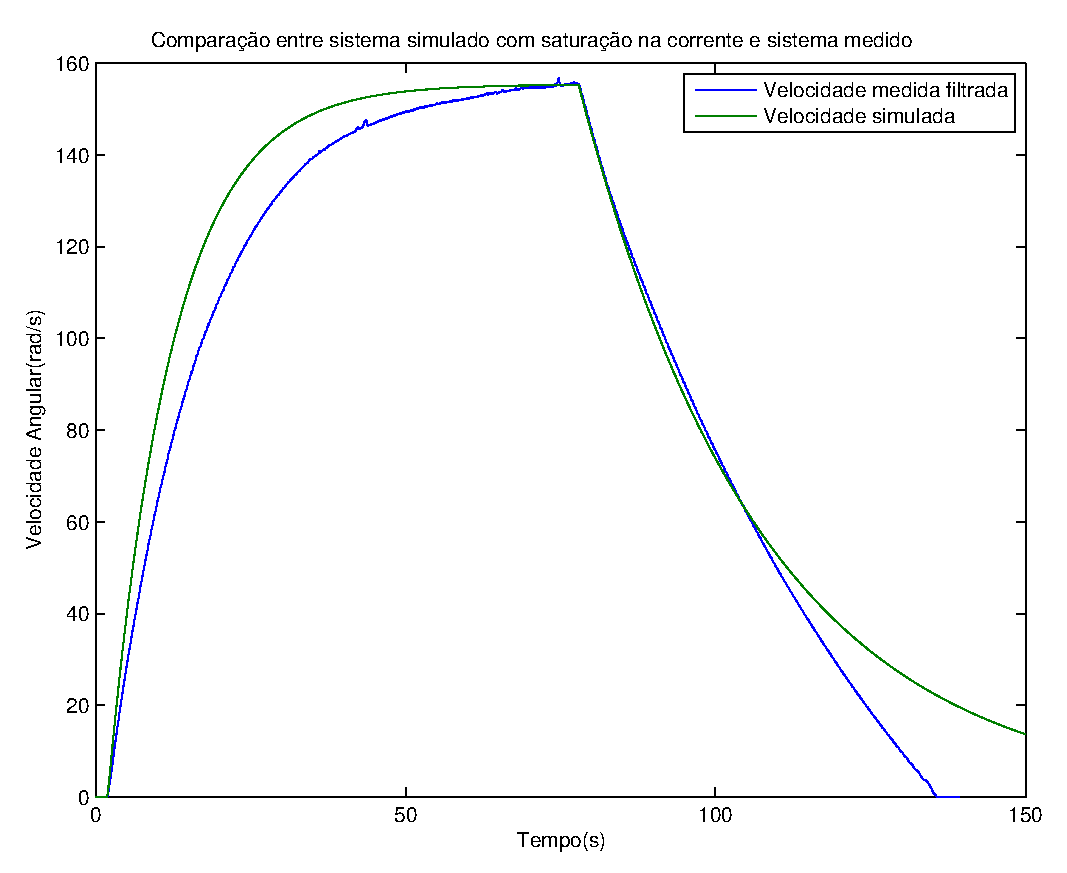
\includegraphics[width=0.8\linewidth]{../simvsat}
	\caption{Comparação entre velocidade angular medida e simulada}
	\label{fig:simvsat}
\end{figure}

Esse novo resultado, representa melhor o sistema e mostra que a aproximação feita para $J$ é razoável, embora ainda não ideal.

\begin{thebibliography}{widestlabel}
	\bibitem{bb:roteiro}{Roteiro do experimento disponibilizado para os alunos}
\end{thebibliography}
\end{document}

